\documentclass[12pt]{article}
    \usepackage{amsfonts,amsmath,amssymb}
    \usepackage{amsmath,multicol,eso-pic}
    \usepackage[utf8]{inputenc}
    \usepackage[T1]{fontenc}
    \usepackage[left=2.00cm, right=2.00cm, top=2.00cm, bottom=2.00cm]{geometry}
    \usepackage{titlesec}
    \usepackage{enumerate}
    \usepackage{multirow}
    \usepackage{graphicx}
    \usepackage{breqn}
    \usepackage[utf8]{inputenc}
    \usepackage{tikz}
    \usepackage{rotating}
    \usepackage{tikz}
    \usetikzlibrary{automata, positioning}
    %\renewcommand{\wedge}{~}
    %\renewcommand{\neg}{\overline}
    \titleformat{\section}{\large}{\thesection.}{1em}{}
    
    
    % % % % % POPUNITE PODATKE
    
    \newcommand{\prezimeIme}{Hamzić Huso}
    \newcommand{\brIndexa}{18305}
    \newcommand{\brZadace}{3}
    
    % % % % % 
    
    \begin{document}
    
    \thispagestyle{empty}
    \begin{center}
      \vspace*{1cm}

      \vspace*{2cm}
      {\huge \bf Zadaća \brZadace } \\
      \vspace*{1cm}
      {\Large \bf iz predmeta Diskretna Matematika}

      \vspace*{1.25cm}

      {\Large Prezime i ime: \prezimeIme} \\
      \vspace*{0.5cm}
      {\Large Br. indexa: \brIndexa} \\
      \vspace*{0.5cm}
      {\Large Asistent: Šeila Bećirović} \\
      \vspace*{0.5cm}
      {\Large Grupa: DM2 [Pon 15.00]} \\ 
      
      \vspace*{2cm}
      \renewcommand{\arraystretch}{1.75}
      \begin{tabular}{|c|c|}
    	\hline Zadatak & Bodovi \\
    	\hline 1 &  \\
    	\hline 2 &  \\
    	\hline 3 &  \\
    	\hline 4 &  \\
    	\hline 5 &  \\
    	\hline 6 &  \\
    	\hline 7 &  \\
    	\hline 8 &  \\
    	\hline 9 &  \\
    	\hline
     \end{tabular}

      \vfill


      {\large Elektrotehnički fakultet Sarajevo}

    \end{center}
    \newpage
    \thispagestyle{empty}
    
    
    % % % % % Rješenja zadataka
	\begin{enumerate}
		\item Rješenje zadatka \\
		\\
		Zadatak 1 [0.25 poena] \\
        \\
Neki eksperiment može dovesti do tri moguća događaja $A_1$, $A_2$ ili $A_3$ iz skupa događaja X. Ova tri događaja imaju respektivno vjerovatnoće 0.2, 0.6 i 0.2. Rezultati tog eksperimenta nisu dostupni direktno, ali se može izvesti testni eksperiment koji daje događaje $B_1$, $B_2$, $B_3$, $B_4$ ili $B_5$ iz skupa događaja Y, koji su u određenoj vezi sa događajima $A_1$, $A_2$ i $A_3$. Vjerovatnoće da testni eksperiment rezultira događajem $B_j$, j = 1, 2, 3, 4, 5 ukoliko je izvorni eksperiment rezultirao događajem $A_i$, i = 1, 2, 3 date su u sljedećoj tabeli: \\

\begin{tabular}{|c|c|c|c|c|c|}
\hline
p(${B_j}$/${A_i}$) & ${B_1}$   & ${B_2}$   &  ${B_3}$  & ${B_4}$ & ${B_5}$   \\ \hline
${A_1}$                           & 0.05  & 0.15 & 0.2 & 0.2  & 0.4  \\ \hline
${A_2}$                          & 0.05 & 0.15 & 0.05  & 0.35 & 0.4 \\ \hline
${A_3}$                         & 0.35 & 0.2  & 0.2  & 0.15 & 0.1  \\ \hline
\end{tabular} \\ 
\\ 
\\ 
Odredite entropije skupa izvornih i testnih događaja H(X) i H(Y), uvjetne entropije H(X/Y) i H(Y/X), zajedničku entropiju H(X,Y) te srednju količinu informacije I(X,Y) koju testni događaji nose o izvornim događajima. \\
\\
*Kako već imamo vjerovatnoće događaja X, entropiju H(X) lahko računamo
entropiju H(X):
\begin{equation*}
    H(X) = - \sum_{i = 1}^3 P(X_i) \cdot log_2~(P(X_i))
\end{equation*}
odnosno:
\begin{equation*}
    H(X) = - (0.2 \cdot log_2~0.2 + 0.6 \cdot log_2~0.6 + 0.2 \cdot log_2~0.2) = 1.37095
\end{equation*}

 Kako bi odredili entropiju H(Y) potrebne su nam sve vjerovatnoće P($B_j$) ($j = 1,2,...5)$ a njih lahko računamo : \\
\begin{equation*}
    P(B_1) = 0.2\cdot0.05 + 0.6\cdot0.05 + 0.2\cdot0.35 = 0.11 
\quad P(B_2) = 0.2\cdot0.15 + 0.6\cdot0.15 + 0.2\cdot0.2 = 0.16
\end{equation*}
\begin{equation*}
    P(B_3) = 0.2\cdot0.2 + 0.6\cdot0.05 + 0.2\cdot0.2=0.11
    \quad P(B_4) = 0.2\cdot0.2 + 0.6\cdot0.35 + 0.2\cdot0.15=0.28
\end{equation*}
\begin{equation*}
    P(B_5) = 0.2\cdot0.4 + 0.6\cdot0.4 + 0.2\cdot0.1=0.34
\end{equation*}
\vspace{0.25cm}
Sada možemo izračunati H(Y):
\begin{equation*}
    H(Y) = - \sum_{j = 1}^5 P(B_j) \cdot log_2~(P(B_j))
\end{equation*}
odnosno:
\begin{equation*}
    H(Y) = - (0.11 \cdot log_2~0.11 + 0.16 \cdot log_2~0.16 + 0.11 \cdot log_2~0.11
    + 0.28 \cdot log_2~0.28 + 0.34 \cdot log_2~0.34)
\end{equation*}
odnosno:
\begin{equation*}
    \fbox{H(Y) = 2.166}
\end{equation*}
H(X,Y) ćemo izračunati pomoću tabele, odnosno:\\
\begin{equation*}
    H(X,Y) = - \sum_{j = 1}^5\sum_{i = 1}^3 P(B_jA_i) \cdot log_2~(P(B_jA_i)) = 3.364
\end{equation*}
Sad ćemo izračunati H(X/Y), H(Y/X), I(X,Y):
\begin{equation*}
    H(X/Y) = H(X,Y) - H(Y) = 3.364 - 2.166 = 1.198
\end{equation*}
\begin{equation*}
    H(Y/X) = H(X,Y) - H(X) = 3.364 - 1.37 = 1.994
\end{equation*}
\begin{equation*}
    I(X,Y) = H(X) - H(X/Y) = 1.37095 + 2.166 - 3.364 = 0.172
\end{equation*}
		\item Rješenje zadatka \\
		\\
		Zadatak 2 [0.25 poena] \\
        \\
Na nekom fakultetu, troškove studija za 33\% studenata plaća država, dok su ostali studenti samofinansirajući. Među studentima koji se školuju o trošku države, 47\% studenata stanuje u studentskom domu, dok među samofinansirajućim studentima 39\% studenata stanuje u studentskom domu. Svi studenti koji stanuju u studentskom domu ujedno posjeduju i iskaznicu za subvencionirani javni prevoz, dok među studentima koji ne stanuju u studentskom domu istu iskaznicu posjeduje i 47\% studenata čiji studij plaća država te 45\% samofinansirajućih studenata.
\\
Odredite koliku prosječnu količinu informacije saznanje o tome posjeduje li student iskaznicu za subvencionirani javni prenos ili ne nosi o načinu finansiranja njegovog studija (tj. da li ga finansira država ili troškove snosi sam). \\
\\

 Skup sa događajima "troškove studija studenta plaća država" i "student je samofinansirajući" označimo sa X, pri čemu je prvi događaj $X_1$ a drugi događaj $X_2$. Na osnovu teksta zadatka,
poznato je da za ove događaje vrijedi da je 
\begin{equation*}
    p(X_1) = 0.33 \quad p(X_2) = 0.67
\end{equation*}

Analogno neka je Y skup događaja gdje sada $Y_1$ predstavlja događaj "student stanuje u studenskom domu" a $Y_2$ "student ne stanuje u studentskom domu". Pa imamo uslovne vjerovatnoće:

\begin{equation*}
    p(Y_1/X_1) = 0.47 \quad p(Y_1/X_2) = 0.39
\end{equation*}
		
Moraju biti zadovoljene sljedeće jednakosti jer student kojeg država financira može ili da živi ili da ne živi u studentskom domu(isto ovo vrijedi i za samofinansirajuće studente). Pa imamo jednakosti:
\begin{equation*}
    p(Y_1/X_1) + p(Y_2/X_1) = 1 \quad p(Y_1/X_2) + p(Y_2/X_2) = 1
\end{equation*}
na osnovu čega se mogu izračunati sljedeće uslovne vjerovatnoće
\begin{equation*}
    p(Y_2/X_1) = 1 - p(Y_1/X_1) = 0.53 \quad p(Y_2/X_2) = 1 - p(Y_1/X_2) = 0.61
\end{equation*}
Neka je sad Z skup događaja koji sadrži događaje $Z_1$ - "student posjeduje iskaznicu za javni prevoz" i $Z_2$ - "student ne posjeduje iskaznicu za javni prevoz".
Pa možemo odrediti vjerovatnoće: \\
p($Z_1$/$X_1$) = $0.47 + 0.47\cdot(1 - 0.47) = 0.7191$.  Jasno je da svaki student čije troškove studija plaća
država ili ima ili nema iskaznicu, pa je vjerovatnoća p($Z_2$/$X_1$) = 1 - 0.7191 = 0.2809
\\
\\
Na sličan način računa se vjerovatnoća da student posjeduje iskaznicu uz uslov da je on samofinansirajući, te ona iznosi 0.39 + 0.45 ${\cdot}$ (1 - 0.39) = 0.6645. Ovo je naša uvjetna vjerovatnoća p($Z_1$/$X_2$), odnosno njena suprotna vjerovatnoća je p($Z_2$/$X_2$) = 1 - 0.6645 = 0.3355. Formirajmo tabelu za dobijene vrijednosti \\
\\
\begin{tabular}{|c|c|c|c|c|c|}
\hline
p(${Z_j}$/${X_i}$) & ${Z_1}$   &  ${Z_2}$ \\ \hline
${X_1}$                           & 0.7191  & 0.2809 \\ \hline
${X_2}$                          & 0.6645 & 0.3355 \\ \hline
\end{tabular} \\

Prosječna količina informacija koju informacija da li student posjeduje iskaznicu za
subvencionirani javni prevoz ili ne nosi o načinu finansiranja njegovog studija označava se sa
I(X, Z) i računa se kao:
\begin{equation*}
    I(X,Z) = H(X) + H(Z) - H(X,Z)
\end{equation*}
Nađimo H(X) kao:
\begin{equation*}
    H(X) = - (p(X_1) \cdot log_2~p(X_1) + p(X_2) \cdot log_2~p(X_2)) = -(0.33 \cdot log_2~0.33 + 0.67 \cdot log_2~0.67) = 0.91492
\end{equation*}

Analogno H(Z):
\begin{equation*}
    H(Z) = - (p(Z_1) \cdot log_2~p(Z_1) + p(Z_2) \cdot log_2~p(Z_2))
\end{equation*}
Ali vjerovatnoće p($Z_1$) i p($Z_2$) nisu poznate, međutim lahko ih računamo:
\begin{equation*}
    p(Z_1) = p(X_1) \cdot p(Z_1/X_1) + p(X_2) \cdot p(Z_1/X_2) = 0.33 \cdot 0.7191 + 0.67 \cdot 0.6645 = 0.6825
\end{equation*}
\begin{equation*}
    p(Z_2) = 1 - p(Z_1) = 0.3175
\end{equation*}
Entropiju H(Z) sada možemo izračunati:
\begin{equation*}
    H(Z) = - (0.6825 \cdot log_2~0.6825 + 0.3175 \cdot log_2~0.3175) = 0.901
\end{equation*}
Izračunajmo H(X,Z):
\begin{equation*}
    H(X,Z) = - (p(X_1Z_1) \cdot log_2~p(X_1Z_1) + p(X_2Z_1) \cdot log_2~p(X_2Z_1)~+
\end{equation*}
\begin{equation*}
    p(X_1Z_2) \cdot log_2~p(X_1Z_2) + p(X_2Z_2) \cdot log_2~p(X_2Z_2))
\end{equation*}
\begin{equation*}
    H(X,Z) = - (0.33 \cdot 0.7191\cdot log_2~(0.33 \cdot 0.7191) + 0.33 \cdot 0.2809\cdot log_2~(0.33 \cdot 0.2809)+
\end{equation*}
\begin{equation*}
   +0.67\cdot0.6645\cdot log_2~( 0.67\cdot0.6645) + 0.67\cdot0.3355\cdot log_2~(0.67\cdot0.3355) = 1.8137
\end{equation*}
I na kraju imamo: 
\begin{equation*}
    \fbox{I(X,Z) = H(X) + H(Z) - H(X,Z) = 0.91492 + 0.901- 1.8137 = 0.00222}
\end{equation*}
		\item Rješenje zadatka \\
		\\
		Zadatak 3 [0.35 poena] \\

Markovljev izvor informacija prvog reda emitira četiri različite poruke a, b, c i d. Ovisno od toga koja je poruka posljednja emitirana, izvor se nalazi u jednom od 4 moguća stanja Sa, Sb, Sc i Sd koja redom odgovaraju emitiranim porukama a, b, c odnosno d. Vjerovatnoće da će izvor emitirati neku od ove 4 poruke ovisno od stanja u kojem se nalazi date su u sljedećoj tablici: \\

\begin{tabular}{|c|c|c|c|c|c|}
\hline
p(${x_j}$ / ${S_i}$) & a    & b    & c    & d    \\ \hline
${S_a}$        & 0.2  & 0.4  & 0.25  & 0.15  \\ \hline
${S_b}$        & 0.15 & 0.05 & 0.3 & 0.5 \\ \hline
${S_c}$        & 0.25 & 0.05  & 0.4 & 0.3  \\ \hline
${S_d}$        & 0.1 & 0.05 & 0.45  & 0.4  \\ \hline
\end{tabular} \\
\\
\\
Odredite entropiju i redudansu ovog izvora, zatim entropiju sekvenci dužine 7 te vjerovatnoću pojave sekvence bcbcdbbc.

\vspace{0.5cm}
Izvor možemo modelirati pomoću 4 stanja,
$S_a$, $S_b$, $S_c$, $S_d$ koja redom odgovaraju prethodno emitiranim porukama a, b, c, d. 
Grafički prikaz konačnog automata koji modelira ovaj izvor dat je na slici
ispod:	\\
\\
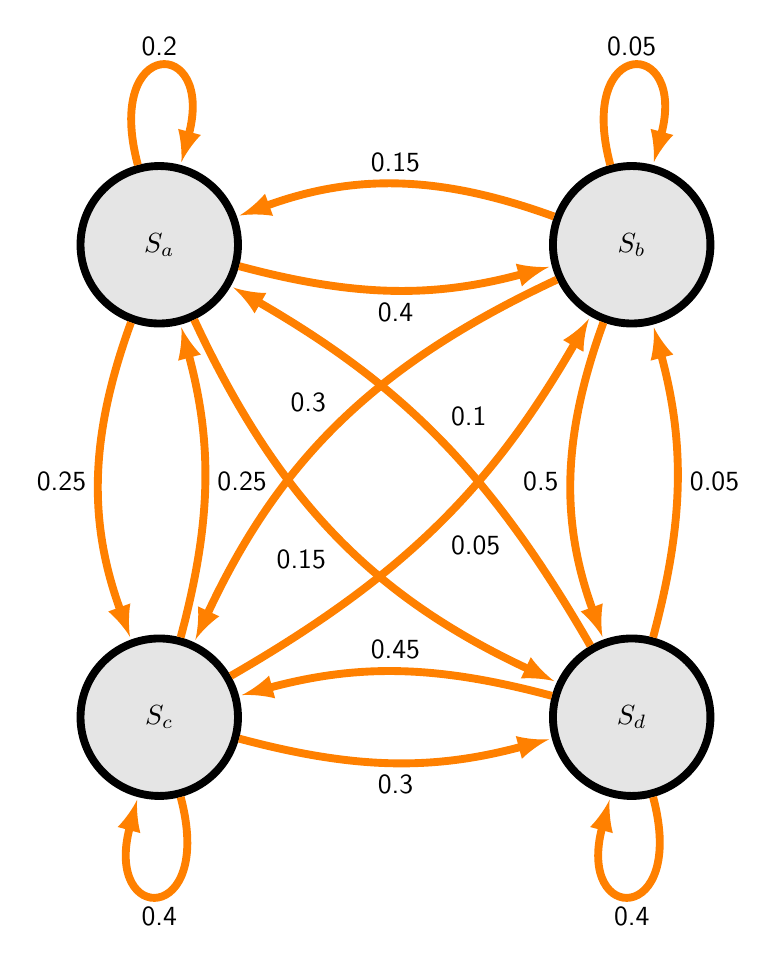
\begin{tikzpicture}[font=\sffamily]
        % Setup the style for the states
        \tikzset{node style/.style={state, 
                                    minimum width=2cm,
                                    line width=1mm,
                                    fill=gray!20!white}}
 
        % Draw the states
        \node[node style] at (0, 0)     (bull)     {${S_c}$};
        \node[node style] at (6, 0)     (bear)     {${S_d}$};
        \node[node style] at (0, 6) (stagnant) {${S_a}$};
        \node[node style] at (6, 6) (masha) {${S_b}$};
        
        % Connect the states with arrows
        \draw[every loop,
              auto=right,
              line width=1mm,
              >=latex,
              draw=orange,
              fill=orange]
            (stagnant)     edge[loop above]               node {0.2} (stagnant)
            (stagnant)     edge[bend right=15]            node {0.4} (masha)
            (stagnant)     edge[bend right=20]            node {0.25} (bull)
            (stagnant)     edge[bend right=20]            node {0.15} (bear)
            (masha)     edge[bend right=20]            node {0.15} (stagnant)
            (masha)     edge[loop above]               node {0.05} (bear)
            (masha)     edge[bend right=20]            node {0.3} (bull)
            (masha)     edge[bend right=20]            node {0.5} (bear)
            (bull)     edge[bend right=15]            node {0.25} (stagnant)
            (bull)     edge[bend right=15]            node {0.05} (masha)
            (bull)     edge[loop below]            node {0.4} (bull)
            (bull)     edge[bend right=15]            node {0.3} (bear)
            (bear)     edge[bend right=15]            node {0.1} (stagnant)
            (bear)     edge[bend right=15]            node {0.05} (masha)
            (bear)     edge[bend right=15]            node {0.45} (bull)
            (bear)     edge[loop below]            node {0.4} (bear);
\end{tikzpicture}
\\
\\
Stanje $S_a$ može nastati prelazom iz stanja $S_a$, $S_b$, $S_c$ ili $S_d$ svaki put uz
emitiranje poruke a. Na osnovu teoreme o totalnoj vjerovatnoći za svako stanje, imamo sisteme:

\begin{equation*}
    P(S_a) = 0.2 \cdot P(S_a) + 0.15 \cdot P(S_b) + 0.25 \cdot P(S_c) + 0.1 \cdot P(S_d)
\end{equation*}
\begin{equation*}
    P(S_b) = 0.4 \cdot P(S_a) + 0.05 \cdot P(S_b) + 0.05 \cdot P(S_c) + 0.05 \cdot P(S_d)
\end{equation*}
\begin{equation*}
    P(S_c) = 0.25 \cdot P(S_a) + 0.3 \cdot P(S_b) + 0.4 \cdot P(S_c) + 0.45 \cdot P(S_d)
\end{equation*}
\begin{equation*}
    P(S_a) + P(S_b) + P(S_c) + P(S_d) = 1
\end{equation*}
Rješenja našeg sistema su respektivno:
\begin{equation*}
    \fbox{P($S_a$) = 0.18} \quad \fbox{P($S_b$) = 0.113} \quad \fbox{P($S_c$) = 0.378} \quad \fbox{P($S_d$) = 0.3284}
\end{equation*}

Da bi odredili entropiju izvora H(X/$X^{\infty}$) moramo odrediti entropije pojedinih stanja, odnosno H($S_a$), H($S_b$), H($S_c$), H($S_d$):
\begin{equation*}
    H(S_a) =  - (P(a/S_a) \cdot log_2~P(a/S_a) + P(b/S_a) \cdot log_2~P(b/S_a)~+
\end{equation*}
\begin{equation*}
    P(c/S_a) \cdot log_2~P(c/S_a) + P(d/S_a) \cdot log_2~P(d/S_a))
\end{equation*}
analogno je i za ostala stanja pa ćemo napisati samo rješenja jer se ovo uz pomoć grafika lahko računa
\begin{equation*}
    \fbox{H($S_a$) = 1.9037} \quad \fbox{H($S_b$) = 1.6477} \quad \fbox{H($S_c$) = 1.7659} \quad \fbox{H($S_d$) = 1.5954}
\end{equation*}
Za entropiju izraza imamo:
\begin{equation*}
    H(X/X^\infty) = P(S_a)H(S_a) + P(S_b)H(S_b) + P(S_c)H(S_c) + P(S_d)H(S_d) = 1.7202
\end{equation*}
Redudansu izvora računamo kao:
\begin{equation*}
    R = \frac{log_2~4 - H(X/X^\infty)}{log_2~4} = \frac{2 - 1.7202}{2} = 0.1399
\end{equation*}
Vjerovatnoću sekvence ${\boldsymbol{bcbcdbbc}}$ možemo izračunati kao
\begin{equation*}
    P(bcbcdbbc) = P(b) \cdot P(c/b) \cdot P(b/c) \cdot P(c/b) \cdot P(d/c) \cdot P(b/d) \cdot P(b/b) \cdot P(c/b)
\end{equation*}
odnosno 
\begin{equation*}
    0.113 \cdot 0.3 \cdot 0.05 \cdot 0.3 \cdot 0.3 \cdot 0.05 \cdot 0.05 \cdot 0.3 = 1.144 \cdot 10^{-7}
\end{equation*}
Za računanje entropije sekvenci dužine 7 imamo relaciju:
\begin{equation*}
    H(X^7) = H(X^1) + 6 \cdot H(X/X^\infty) 
\end{equation*}
Treba nam još entropija H($X^1$):
\begin{equation*}
    H(X^1) = -(P(a) \cdot log_2~P(a) + P(b) \cdot log_2~P(b) + P(c) \cdot log_2~P(c) + P(d) \cdot log_2~P(d)) = 1.8588
\end{equation*}
Izračunajmo sada entropiju sekvenci 7:
\begin{equation*}
    H(X^7) = H(X^1) + 6 \cdot H(X/X^\infty)  = 1.8588 + 6 \cdot 1.7202 = 12.18
\end{equation*}
		\item Rješenje zadatka \\
		\\
Zadatak 4 [0.4 poena] \\
\\
Markovljev izvor informacija drugog reda emitira dvije različite poruke 0 i 1. Ovisno od toga koje su dvije poruke posljednje emitirane, izvor se može naći u jednom od 4 moguća stanja $S_{00}$, $S_{01}$, $S_{10}$ odnosno $S_{11}$ (recimo, ukoliko su posljednje dvije emitirane poruke 0 i 1 tim redom, izvor će se nalaziti u stanju $S_{01}$). Vjerovatnoće emitiranja poruke 0 u svakom od tih stanja iznose: \\
\\
\begin{equation*}
    p(0/S_{00}) = 0.4 \quad p(0/S_{01}) = 0.3 \quad p(0/S_{10}) = 0.7 \quad p(0/S_{11}) = 0.1 
\end{equation*}
\\
Odredite entropiju i redudansu ovog izvora, zatim entropiju sekvenci dužine 5 te vjerovatnoću pojave sekvence 111001.

		* Kako je red izvora r = 2, izvor možemo modelirati pomoću 4 stanja $S_{00}$,
$S_{01}$, $S_{10}$ odnosno $S_{11}$. Grafički prikaz konačnog automata koji modelira ovaj
izvor prikazan je na slici ispod: \\
\\
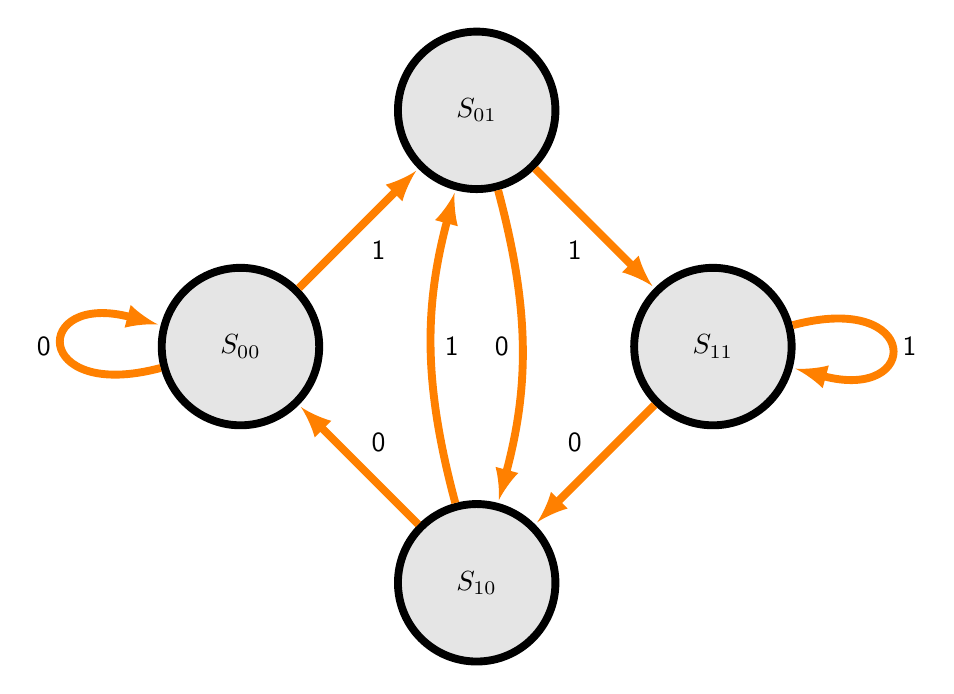
\begin{tikzpicture}[font=\sffamily]
        % Setup the style for the states
        \tikzset{node style/.style={state, 
                                    minimum width=2cm,
                                    line width=1mm,
                                    fill=gray!20!white}}
 
        % Draw the states
        \node[node style] at (0, 3)     (bull)     {${S_{00}}$};
        \node[node style] at (3, 0)     (bear)     {${S_{10}}$};
        \node[node style] at (3, 6) (stagnant) {${S_{01}}$};
        \node[node style] at (6, 3) (masha) {${S_{11}}$};
        
        % Connect the states with arrows
        \draw[every loop,
              auto=right,
              line width=1mm,
              >=latex,
              draw=orange,
              fill=orange]
            (stagnant)     edge[bend right=0]            node {1} (masha)
            (stagnant)     edge[bend left=15]            node {0} (bear)
            (bull)     edge[loop left]            node {0} (bull)
            (bull)     edge[bend left=0]            node {1} (stagnant)
            (masha)     edge[loop right]            node {1} (masha)
            (masha)     edge[bend left=0]            node {0} (bear)
            (bear)     edge[bend left=15]            node {1} (stagnant)
            (bear)     edge[bend right=0]            node {0} (bull);
\end{tikzpicture}
\\
Kako imamo vjerovatnoće emitiranja poruke 0 u svim stanjima, na osnovu
njih možemo dobiti vjerovatnoće emitiranja poruke 1 u tim istim stanjima:
\begin{equation*}
    p(1/S_{00}) = 0.6 \quad p(1/S_{01}) = 0.7 \quad p(1/S_{10}) = 0.3 \quad p(1/S_{11}) = 0.9 
\end{equation*}
Izračunajmo entropiju stanja: \\
\begin{equation*}
    H(S_{00}) = -(0.4 \cdot log_2~0.4 + 0.6 \cdot log_2~0.6) = 0.9709
\end{equation*}
\begin{equation*}
    H(S_{01}) = -(0.3 \cdot log_2~0.3 + 0.7 \cdot log_2~0.7) = 0.881
\end{equation*}
\begin{equation*}
    H(S_{10}) = -(0.7 \cdot log_2~0.7 + 0.3 \cdot log_2~0.3) = 0.881
\end{equation*}
\begin{equation*}
    H(S_{11}) = -(0.1 \cdot log_2~0.1 + 0.9 \cdot log_2~0.9) = 0.4689
\end{equation*}
Sada možemo postaviti sistem jednačina pomoću kojeg dobijamo vjerovatnoće svakog od stanja:
\begin{equation*}
    P(S_{00}) = 0.4 \cdot P(S_{00}) + 0.7 \cdot P(S_{10})
\end{equation*}
\begin{equation*}
    P(S_{01}) = 0.6 \cdot P(S_{00}) + 0.3 \cdot P(S_{10})
\end{equation*}
\begin{equation*}
    P(S_{11}) = 0.7 \cdot P(S_{01}) + 0.9 \cdot P(S_{11})
\end{equation*}
\begin{equation*}
    P(S_{00}) + P(S_{01}) + P(S_{10}) + P(S_{11}) = 1
\end{equation*}
Respektivno, rješenja su:
\begin{equation*}
    P(S_{00}) = 0.1147 \quad P(S_{01}) = 0.0983 \quad P(S_{10}) = 0.0983\quad P(S_{11}) = 0.6885
\end{equation*}
Izračunajmo sada entropiju izvora
\begin{equation*}
    H(X/X^\infty) = P(S_{00})H(S_{00}) + P(S_{01})H(S_{01}) + P(S_{10})H(S_{10}) + P(S_{11})H(S_{11}) = 0.6074
\end{equation*} 

Redudansa izvora je:
\begin{equation*}
    R =  \frac{log_2~2 - 0.6074}{1} = 0.39259
\end{equation*}
Odredimo entropiju sekvenci dužine 5:
\begin{equation*}
    H(X^5) = H(X^2) + 3 \cdot H(X/X^\infty) 
\end{equation*}
Odredimo $H(X^2)$:
\begin{equation*}
    H(X^2) = -(P(S_{00}) \cdot log_2~P(S_{00}) + P(S_{01}) \cdot log_2~P(S_{01}) +
    P(S_{10}) \cdot log_2~P(S_{10}) + P(S_{11}) \cdot log_2~P(S_{11}))
\end{equation*}
odnosno
\begin{equation*}
    H(X^2) = 1.38702
\end{equation*}
odnosno entropija sekvenci 5 je:
\begin{equation*}
    H(X^5) = H(X^2) + 3 \cdot H(X/X^\infty) = 1.38702 + 3 \cdot 0.6074 = 3.20922
\end{equation*}
Izračunajmo još i vjerovatnoću sekvence 111001:
\begin{equation*}
    p(111001) = p(11) \cdot p(1/11) \cdot p(0/11) \cdot p(0/10) \cdot p(1/00) = 0.6885 \cdot 0.9 \cdot 0.1 \cdot 0.7 \cdot 0.6 = 0.0260253
\end{equation*}
odnosno 
\begin{equation*}
   \fbox{p(111001) = 2.60253\%}
\end{equation*}
		\item Rješenje zadatka \\
		\\
		Zadatak 5 [0.6 poena] \\
        \\
Ergodični izvor informacija bez memorije emitira 10 poruka A, B, C, D, E, F, G, H, I i J. Proučavanjem sekvence dužine 449 koju je emitirao ovaj izvor, uočena je sljedeća učestalost pojavljivanja pojedinih poruka: \\
\\
\begin{tabular}{|c|c|c|c|c|c|c|c|c|c|c|}
\hline
Poruka:     & A  & B  & C  & D  & E  & F  & G  & H  & I  & J  \\ \hline
Učestalost: & 39 & 77 & 30 & 69 & 49 & 25 & 82 & 28 & 10 & 40 \\ \hline
\end{tabular}
\\
\\
Za ovaj izvor informacija formirajte: \\
\\
a. Binarni Shannon-Fano kod sa simbolima 0 i 1; \\
b. Binarni Huffmanov kod sa simbolima 0 i 1; \\
c. Ternarni Huffmanov kod sa simbolima 0, 1 i 2. \\

Za sva tri načina kodiranja, izračunajte protok informacija kroz komunikacioni kanal, procenat iskorištenja kanala veze, te kodirajte sekvencu poruka BFHIAEDIB.

		* a)~Konstrukcija Shannon-Fano koda prikazana je u sljedećoj tabeli, pri
čemu su u tabeli umjesto vjerovatnoća prikazane učestalosti, što se
zapravo svodi na isto, jer su učestalosti proporcionalne vjerovatnoćama. \\
\\
\begin{tabular}{|l|l|l|llllllll}
\cline{1-3}
82 G &       & \textbf{82/00} &                                      &                                       &  &  &  &  &  &  \\ \cline{1-1} \cline{3-4}
77 B & 228/0 & 146/01         & \multicolumn{1}{l|}{\textbf{77/010}} &                                       &  &  &  &  &  &  \\ \cline{1-1} \cline{4-4}
69 D &       &                & \multicolumn{1}{l|}{\textbf{69/011}} &                                       &  &  &  &  &  &  \\ \cline{1-4}
49 E &       &                & \multicolumn{1}{l|}{\textbf{49/100}} &                                       &  &  &  &  &  &  \\ \cline{1-1} \cline{4-5}
40 J &       & 128/10         & \multicolumn{1}{l|}{79/101}          & \multicolumn{1}{l|}{\textbf{40/1010}} &  &  &  &  &  &  \\ \cline{1-1} \cline{5-5}
39 A &       &                & \multicolumn{1}{l|}{}                & \multicolumn{1}{l|}{\textbf{39/1011}} &  &  &  &  &  &  \\ \cline{1-1} \cline{3-5}
30 C & 221/1 &                & \multicolumn{1}{l|}{58/110}          & \multicolumn{1}{l|}{\textbf{30/1100}} &  &  &  &  &  &  \\ \cline{1-1} \cline{5-5}
28 H &       & 93/11         & \multicolumn{1}{l|}{}                & \multicolumn{1}{l|}{\textbf{28/1101}} &  &  &  &  &  &  \\ \cline{1-1} \cline{4-5}
25 F &       &                & \multicolumn{1}{l|}{35/111}          & \multicolumn{1}{l|}{\textbf{25/1110}} &  &  &  &  &  &  \\ \cline{1-1} \cline{5-5}
10 I &       &                & \multicolumn{1}{l|}{}                & \multicolumn{1}{l|}{\textbf{10/1111}} &  &  &  &  &  &  \\ \cline{1-5}
\end{tabular}
\\
\\
Imamo kodirane sekvence:
\begin{equation*}
    A - 1011 \quad B - 010 \quad C - 1100 \quad D - 011 \quad E - 100 \quad F - 1110 \quad G - 00 \quad H - 1101 \quad I - 1111 \quad J - 1010
\end{equation*}
Izračunajmo H(X/${X^\infty}$) pri čemu sad moramo uzeti vjerovatnoće u obzir, \\odnosno  učestalost / 449:
		
\begin{equation*}
    H(X/X^\infty) = - \frac{1}{449}(82 \cdot log_2~\frac{82}{449} +	77 \cdot log_2~\frac{77}{449} +
    69 \cdot log_2~\frac{69}{449} + 49 \cdot log_2~\frac{49}{449} + 40 \cdot log_2~\frac{40}{449}~+
\end{equation*}
\begin{equation*}
	39 \cdot log_2~\frac{39}{449} + 30 \cdot log_2~\frac{30}{449} + 28 \cdot log_2~\frac{28}{449} +
	25 \cdot log_2~\frac{25}{449} + 10 \cdot log_2~\frac{10}{449})
\end{equation*}
odnosno:
\begin{equation*}
    H(X/X^\infty) = 3.1281
\end{equation*}
Da bi izračunali prosječnu dužinu kodne riječi, ukoliko je $n_i$ dužina
kodne riječi pridružene i-toj poruci koristimo formulu:
\begin{equation*}
    n_{sr} = \frac{1}{N} \cdot \sum_{i = 1}^m N_i \cdot n_i
\end{equation*}
odnosno:
\begin{equation*}
    n_{sr} = \frac{1}{449}(82 \cdot 2 + 77 \cdot 3 + 69 \cdot 3 + 49 \cdot 3 + 40 \cdot 4 + 39 \cdot 4 + 30 \cdot 4 + 28 \cdot 4 + 25 \cdot 4 + 10 \cdot 4) = 3.200
\end{equation*}
pa je protok informacija:
\begin{equation*}
    \overline{I(X)} = \frac{H(X/X^\infty)}{n_{sr} \cdot \tau} = \frac{0.97753125}{\tau}
\end{equation*}
odakle slijedi da je iskorištenost kanala veze približno 97.753\% \\
\\
Kodirana poruka BFHIAEDIB glasi (razmak između svakog slova): \\
010 1110 1101 1111 1011 100 011 1111 010
\vspace{0.5cm}	
\\
b) Binarni Huffmanov kod sa 0 i 1: \\

\begin{figure}[htp]
    \centering
    \includegraphics[width=15cm]{5b.png}
\end{figure}


 Po formuli koju smo koristili u dijelu zadatka pod a, dobijamo da je:
\begin{equation*}
    n_{sr} = \frac{1}{449}(3 \cdot 77 + 4 \cdot 39 + 5 \cdot 25 + 5 \cdot 10 + 3 \cdot 69 +
    4 \cdot 30 + 4 \cdot 28 + 3 \cdot 49 + 3 \cdot 40 + 2 \cdot 82) = 3.189
\end{equation*}
pa je na osnovu toga protok informacija (pošto je entropija izvora ista kako pod a)\\
\begin{equation*}
    \overline{I(X)} = \frac{H(X/X^\infty)}{n_{sr} \cdot \tau} = \frac{0.9809}{\tau}
\end{equation*}
odakle slijedi da je iskorištenost kanala veze približno 98.09\% \\


Kodirana poruka BFHIAEDIB glasi (razmak između svakog slova): \\
000 00110 0111 00111 0010 100 010 00111 000 \\

c) Ternarni Huffmanov kod sa 0, 1 i 2 : \\

\begin{figure}[htp]
    \centering
    \includegraphics[width=9cm]{5c.png}
\end{figure}

Na isti način kao u dijelovima zadatka pod a i b dobijamo da je:
\begin{equation*}
    n_{sr} = \frac{1}{449}(2 \cdot 82 + 2 \cdot 77 + 2 \cdot 69 + 2 \cdot 49 + 2 \cdot 40 +
    2 \cdot 39 + 3 \cdot 25 + 3 \cdot 10 + 2 \cdot 30 + 2 \cdot 28) = 2.0779
\end{equation*}
Entropija nam je ista kao i pod a odnosno b, jer je isti skup podataka, pa na osnovu toga imamo protok informacija:
\begin{equation*}
    \overline{I(X)} = \frac{H(X/X^\infty)}{n_{sr} \cdot \tau} = \frac{1.5054}{\tau}
\end{equation*}
Kako je kapacitet kanala veze $C_c$ = ${\frac{log_2 3}{\tau}}$ = ${\frac{1.5850}{\tau}}$ iskorištenost kanala veze je \\ ${\frac{1.5054}{1.5850}}$ = 0.9498 = 94.98\% \\
\\
Kodirana poruka BFHIAEDIB glasi (razmak između svakog slova): \\
01 200 22 201 12 10 02 201 01 
\newpage
		\item Rješenje zadatka \\
		\\
		Zadatak 6 [0.7 poena] \\
        \\
Izvor informacija bez memorije emitira 4 poruke A, B, C i D. Vjerovatnoće pojavljivanja ovih poruka iznose:
\\
\\
p(A) = 0.25 \\
p(B) = 0.05 \\
p(C) = 0.45 \\
p(D) = 0.25 \\
\\
Za ovaj izvor informacija formirajte \\
a. Binarni Shannon-Fano kod sa simbolima 0 i 1, \\
b. Binarni Huffmanov kod sa simbolima 0 i 1, \\
c. Binarni Shannon-Fano kod sa simbolima 0 i 1, ali kodirajući parove poruka umjesto individualnih poruka, \\
d. Binarni Huffmanov kod sa simbolima 0 i 1, ali kodirajući parove poruka umjesto individualnih poruka. \\
\\
Za sva četiri načina kodiranja, izračunajte protok informacija kroz komunikacioni kanal, procenat iskorištenja kanala veze, te kodirajte sekvencu poruka BADCDBCBCB. \\
\\
* a) Binarni Shannon-Fano kod sa simbolima 0 i 1: 
\\

\begin{tabular}{|l|l|ll}
\cline{1-2}
C 0.45 & \textbf{0.45/0} &  &  \\ \cline{1-3}
A 0.25 & \multirow{3}{*}{0.55/1} & \multicolumn{1}{l|}{\textbf{0.25/10}} &  \\ \cline{1-1} \cline{3-4} 
D 0.25 &  & \multicolumn{1}{l|}{\multirow{2}{*}{0.3/11}} & \multicolumn{1}{l|}{\textbf{0.25/110}} \\ \cline{1-1} \cline{4-4} 
B 0.05 &  & \multicolumn{1}{l|}{} & \multicolumn{1}{l|}{\textbf{0.05/111}} \\ \hline
\end{tabular}


Iz tabele se vidi koja je poruka kodirana kojim kodom, izračunajmo entropiju izvora i prosječnu dužinu kodne riječi:
\begin{equation*}
    H(X/X^\infty) = -(0.45 \cdot log_2~0.45 + 0.25 \cdot log_2~0.25 + 0.25 \cdot log_2~0.25 + 0.05 \cdot log_2~ 0.05) = 1.73449
\end{equation*}
\begin{equation*}
    n_{sr} = 0.45 \cdot 1 + 0.25 \cdot 2 + 0.25 \cdot 3 + 0.05 \cdot 3 = 1.85
\end{equation*}
pa je protok kanala veze:
\begin{equation*}
    \overline{I(X)} = \frac{H(X/X^\infty)}{n_{sr} \cdot \tau} = \frac{0.93756}{\tau}
\end{equation*}
odnosno iskorištenost kanala veze je 93.756\%. \\
\\
Kodirana poruka BADCDBCBCB glasi (razmak između svakog slova): \\
111 10 110 0 110 111 0 111 0 111
\newpage

b) Binarni Huffmanov kod sa simbolima 0 i 1:
\\

\begin{tabular}{|l|l|l|c|}
\hline
C 0.45 & C 0.45 & \multirow{3}{*}{\begin{tabular}[c]{@{}l@{}}D/00\\ B/01    0.55\\ A/1\end{tabular}} & \multirow{4}{*}{\textbf{\begin{tabular}[c]{@{}c@{}}D/000\\ B/001\\ A/01\\  C/1\end{tabular}}} \\ \cline{1-2}
A 0.25 & \multirow{2}{*}{\begin{tabular}[c]{@{}l@{}}D/0   0.3\\ B/1\end{tabular}} &  &  \\ \cline{1-1}
D 0.25 &  &  &  \\ \cline{1-3}
B 0.05 & A 0.25 & C 0.45 &  \\ \hline
\end{tabular}\\
\\ 
Iz tabele se može vidjeti kojim su sekvencama slova kodirana. Entropija
je ista kao u dijelu zadatka pod a, a isti je slučaj i sa prosječnom
dužinom kodne rijeći $n_{sr}$ = 1.85, pa vrijede isti zaključci osim kodirane kodirane sekvence.
Odnosno protok kanala veze je:
\begin{equation*}
    \overline{I(X)} = \frac{H(X/X^\infty)}{n_{sr} \cdot \tau} = \frac{0.93756}{\tau}
\end{equation*}
odnosno iskorištenost kanala veze je 93.756\%. \\
\\
Kodirana poruka BADCDBCBCB glasi (razmak između svakog slova): \\
001 01 000 1 000 001 1 001 1 001
\\
\\
c) Binarni Shannon-Fano kod sa simbolima 0 i 1 (parovi poruka): 
\\
\begin{figure}[htp]
    \centering
    \includegraphics[width=17cm]{6c_v2.png}
\end{figure}
\\
\\
Iz tabele se vidi koji su parovi poruka kodirani kojim kodom, izračunajmo
prosječnu dužinu kodne riječi:
\begin{equation*}
    n_{sr} = 0.2025 \cdot 3 + 4 \cdot 0.1125 \cdot 3 + 4\cdot 0.0625 \cdot 4 + 2\cdot0.0225 \cdot 5 +3\cdot 0.0125 \cdot 6 +
    0.0125 \cdot 7 + 0.0025 \cdot 7
\end{equation*}
\begin{equation*}
     n_{sr} = 3.5125
\end{equation*}
Entropija izvora je ovdje faktički entropija sekvenci dužine 2, s obzirom
da ne postoji zavisnost unazad. Pored toga, zbog nepostojanja zavisnosti unazad također vrijedi i \\ H($X^2$) = 2 ${\cdot}$ H(X), tako da za protok
informacija dobijamo
\begin{equation*}
    \overline{I(X)} = \frac{2 \cdot H(X/X^\infty)}{n_{sr} \cdot \tau} = \frac{0.98761}{\tau}
\end{equation*}
odnosno iskorištenost kanala veze je 98.761\%. \\
Kodirana poruka BADCDBCBCB glasi (razmak između svaka 2 slova): \\
1111110 100 111101 11101 11101
\\
\\
d) Binarni Huffmanov kod sa simbolima 0 i 1 (parovi poruka):
\\
\begin{figure}[htp]
    \centering
    \includegraphics[width=18cm]{6d_1.png}
\end{figure}
\\
\newpage

\begin{figure}[htp]
    \centering
    \includegraphics[width=18cm]{6d_2.png}
\end{figure}

Iz tabele se vidi koji su parovi poruka kodirani kojim kodom, izračunajmo
prosječnu dužinu kodne riječi:
\begin{equation*}
    n_{sr} = 0.2025\cdot3 + 4\cdot0.0625\cdot4 + 4\cdot0.1125\cdot3 + 7\cdot0.0125 + 7\cdot0.0025 + 3\cdot6\cdot0.0125
\end{equation*}
\begin{equation*}
    + 2\cdot5\cdot0.0225 = 3.5125
\end{equation*}
Entropija izvora je ovdje faktički entropija sekvenci dužine 2, s obzirom
da ne postoji zavisnost unazad. Pored toga, zbog nepostojanja zavisnosti unazad 
također vrijedi i H($X^2$) = 2 ${\cdot}$ H(X), tako da za protok
informacija dobijamo
\begin{equation*}
    \overline{I(X)} = \frac{2 \cdot H(X/X^\infty)}{n_{sr} \cdot \tau} = \frac{0.98761}{\tau}
\end{equation*}
odnosno iskorištenost kanala veze je 98.761\%. \\
Kodirana poruka BADCDBCBCB glasi (razmak između svaka 2 slova): \\
1110000 110 111010 11111 11111
\\
		\newpage
		\item Rješenje zadatka \\
		\\
		Zadatak 7 [0.8 poena] \\
        \\
Markovljev izvor informacija prvog reda emitira tri različite poruke a, b i c. Ovisno od toga koja je poruka posljednja emitirana, izvor se nalazi u jednom od 3 moguća stanja $S_a$, $S_b$ i $S_c$ koja redom odgovaraju emitiranim porukama a, b odnosno c. Vjerovatnoće da će izvor emitirati neku od ove 3 poruke ovisno od stanja u kojem se nalazi date su u sljedećoj tablici: \\
		
\begin{tabular}{|l|l|l|l|}
\hline
p($x_j$ /$S_i$) & a   & b   & c   \\ \hline
$S_a$        & 0.1 & 0.1 & 0.8 \\ \hline
$S_b$        & 0.2 & 0.1 & 0.7 \\ \hline
$S_c$        & 0.5 & 0.2 & 0.3 \\ \hline
\end{tabular}
\\
\\
\\
Za ovaj izvor informacija formirajte binarni Shannon-Fano kod sa simbolima 0 i 1 \\
a. posmatrajući izvor kao izvor bez memorije; \\
b. posmatrajući izvor kao izvor bez memorije, ali kodirajući parove poruka umjesto individualnih poruka; \\
c. koristeći posebno kodiranje za svako stanje; \\
d. koristeći posebno kodiranje za svako stanje, ali kodirajući parove poruka umjesto individualnih poruka. \\
\\
Za sva četiri načina kodiranja, izračunajte protok informacija kroz komunikacioni kanal, procenat iskorištenja kanala veze, te kodirajte sekvencu poruka bccacccabb. U posljednja dva slučaja, pretpostavite da izvor započinje rad u stanju $S_a$.

* Grafički prikaz konačnog automata koji modelira ovaj izvor dat je na slici
ispod: \\
\\
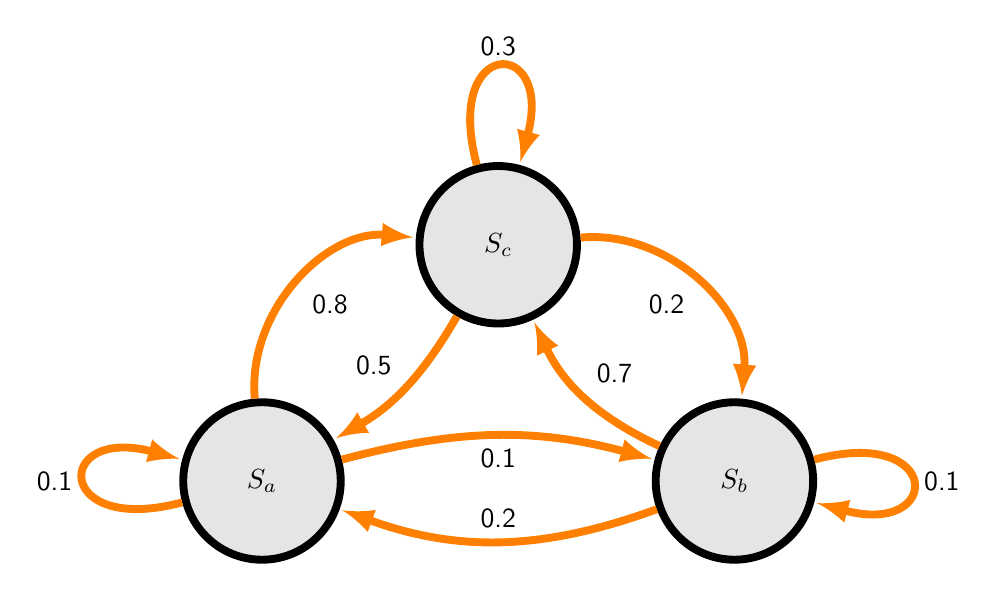
\begin{tikzpicture}[font=\sffamily]
        % Setup the style for the states
        \tikzset{node style/.style={state, 
                                    minimum width=2cm,
                                    line width=1mm,
                                    fill=gray!20!white}}
 
        % Draw the states
        \node[node style] at (0, 3)     (bull)     {${S_{a}}$};
        \node[node style] at (6, 3)     (bear)     {${S_{b}}$};
        \node[node style] at (3, 6) (stagnant) {${S_{c}}$};
        
        % Connect the states with arrows
        \draw[every loop,
              auto=right,
              line width=1mm,
              >=latex,
              draw=orange,
              fill=orange]
            (bull)     edge[loop left]            node {0.1} (bull)
            (stagnant)     edge[loop above]            node {0.3} (stagnant)
            (bear)     edge[loop right]            node {0.1} (bear)
              
            (bear)     edge[bend left=20]            node {0.7} (stagnant)    
            (bear)     edge[bend left=20]            node {0.2} (bull)   
            (bull)     edge[bend left=50]            node {0.8} (stagnant)  
            (bull)     edge[bend left=15]            node {0.1} (bear)    
            (stagnant)     edge[bend left=15]            node {0.5} (bull)  
            (stagnant)     edge[bend left=50]            node {0.2} (bear);
\end{tikzpicture}
\\
\newpage

Na osnovu teoreme o totalnoj vjerovatnoći imamo: \\
\begin{equation*}
    P(S_a) = P(S_a)P(a/S_a) + P(S_b)P(a/S_b) + P(S_c)P(a/S_c)
\end{equation*} 
\begin{equation*}
    P(S_b) = P(S_a)P(b/S_a) + P(S_b)P(b/S_b) + P(S_c)P(b/S_c)
\end{equation*} 
\begin{equation*}
    P(S_a) + P(S_b) + P(S_c) = 1
\end{equation*}
Uvrštavanjem vrijednosti iz tabele iznad dobijamo sistem jednačina čija
su rješenja:
\begin{equation*}
    P(S_a) = 0.3245 \quad P(S_b) = 0.1523 \quad P(S_c) = 0.5231
\end{equation*}
Izračunajmo sada entropije svakog od stanja $S_a$, $S_b$ i $S_c$ čitajući vrijednosti
redova iz tabele i koristeći formulu za entropiju:
\begin{equation*}
    H(S_a) = 0.9219 \quad H(S_b) = 1.1567 \quad H(S_c) = 1.4854
\end{equation*}
Sada možemo izračunati entropiju izvora:
\begin{equation*}
    H(X/X^\infty) = P(S_a)H(S_a) + P(S_b)H(S_b) + P(S_c)H(S_c) = 1.2523
\end{equation*}
- Pređimo sada na kodiranja ($S_a$ -> a, $S_b$ -> b, $S_c$ -> c): \\
\\
a) posmatrajući izvor kao izvor bez memorije:
\\
\\
\begin{tabular}{|l|l|l}
\cline{1-2}
c 0.5231 & \textbf{0.5231/0} &                                            \\ \hline
a 0.3245 & 0.4768/1          & \multicolumn{1}{l|}{\textbf{0.3245/10}} \\ \cline{1-1} \cline{3-3} 
b 0.1523 &                      & \multicolumn{1}{l|}{\textbf{0.1523/11}} \\ \hline
\end{tabular}
\\
\\
Iz tabele se vidi koji su parovi poruka kodirani kojim kodom, izračunajmo
prosječnu dužinu kodne riječi:
\begin{equation*}
    n_{sr} = 0.5231 + 0.3245 \cdot 2 + 0.1523 \cdot 2 = 1.4767
\end{equation*}
samim tim protok je: 
\begin{equation*}
    \overline{I(X)} = \frac{H(X/X^\infty)}{n_{sr} \cdot \tau} = \frac{0.8480}{\tau}
\end{equation*}
odnosno iskorištenost je: 84.80\%. \\
Kodirana poruka bccacccabb glasi (razmak između svakog slova): \\
11 0 0 10 0 0 0 10 11 11
\\
\\
b) posmatrajući izvor kao izvor bez memorije, ali kodirajući parove poruka umjesto individualnih poruka:
\\
\\

\begin{tabular}{|l|l|l|lll}
\cline{1-3}
cc 0.2736 & \multirow{2}{*}{0.4433/0} & \textbf{0.2736/00} &  &  &  \\ \cline{1-1} \cline{3-3}
ac 0.1697 &  & \textbf{0.1697/01} &  &  &  \\ \cline{1-4}
ca 0.1697 & \multirow{7}{*}{0.55619/1} & \multirow{2}{*}{0.275/10} & \multicolumn{1}{l|}{\textbf{0.1697/100}} &  &  \\ \cline{1-1} \cline{4-4}
aa 0.1053 &  &  & \multicolumn{1}{l|}{\textbf{0.1053/101}} &  &  \\ \cline{1-1} \cline{3-5}
bc 0.0796 &  & \multirow{5}{*}{0.281/11} & \multicolumn{1}{l|}{\multirow{2}{*}{0.1592/110}} & \multicolumn{1}{l|}{\textbf{0.0796/1100}} &  \\ \cline{1-1} \cline{5-5}
cb 0.0796 &  &  & \multicolumn{1}{l|}{} & \multicolumn{1}{l|}{\textbf{0.0796/1101}} &  \\ \cline{1-1} \cline{4-5}
ab 0.0494 &  &  & \multicolumn{1}{l|}{\multirow{3}{*}{0.121/111}} & \multicolumn{1}{l|}{\textbf{0.0494/1110}} &  \\ \cline{1-1} \cline{5-6} 
ba 0.0494 &  &  & \multicolumn{1}{l|}{} & \multicolumn{1}{l|}{\multirow{2}{*}{0.07259/1111}} & \multicolumn{1}{l|}{\textbf{0.0494/11110}} \\ \cline{1-1} \cline{6-6} 
bb 0.02319 &  &  & \multicolumn{1}{l|}{} & \multicolumn{1}{l|}{} & \multicolumn{1}{l|}{\textbf{0.02319/11111}} \\ \hline
\end{tabular}
\\
\newpage
Iz tabele se vidi koji su parovi poruka kodirani kojim kodom, izračunajmo
prosječnu dužinu kodne riječi:
\begin{equation*}
    n_{sr} = 0.2736\cdot2 + 0.1697\cdot2 + 0.1697\cdot3 + 0.1053\cdot3 + 2\cdot0.0796\cdot4 + 0.0494\cdot4 + 0.0494\cdot5 + 0.02319\cdot5
\end{equation*}

$n_{sr} = 2.90895$
\\
samim tim protok je: 
\begin{equation*}
    \overline{I(X)} = \frac{2 \cdot H(X/X^\infty)}{n_{sr} \cdot \tau} = \frac{0.8609}{\tau}
\end{equation*}
odnosno iskorištenost je: 86.09\%. \\
Kodirana poruka bccacccabb glasi (razmak između svaka 2 slova): \\
1100 100 00 100 11111
\\
\\
c) koristeći posebno kodiranje za svako stanje:
\\
\\
$S_a$ \\
\\
\begin{tabular}{|l|l|l}
\cline{1-2}
c 0.8 & \textbf{0.8/0} &                                      \\ \hline
b 0.1 & 0.2/1          & \multicolumn{1}{l|}{\textbf{0.1/10}} \\ \cline{1-1} \cline{3-3} 
a 0.1 &                & \multicolumn{1}{l|}{\textbf{0.1/11}} \\ \hline
\end{tabular}
\\
\begin{equation*}
    n_{sr_{a}} = 0.8 + 2\cdot0.1\cdot2 = 1.2
\end{equation*}
 $S_b$ \\
\\
\begin{tabular}{|l|l|l}
\cline{1-2}
c 0.7 & \textbf{0.7/0} &                                      \\ \hline
b 0.2 & 0.3/1          & \multicolumn{1}{l|}{\textbf{0.2/10}} \\ \cline{1-1} \cline{3-3} 
a 0.1 &                & \multicolumn{1}{l|}{\textbf{0.1/11}} \\ \hline
\end{tabular}
\\
\begin{equation*}
    n_{sr_{b}} = 0.7 + 0.2\cdot2 + 0.1\cdot2 = 1.3
\end{equation*}
 $S_c$ \\
\\
\begin{tabular}{|l|l|l}
\cline{1-2}
a 0.5 & \textbf{0.5/0} &                                      \\ \hline
c 0.3 & 0.5/1          & \multicolumn{1}{l|}{\textbf{0.3/10}} \\ \cline{1-1} \cline{3-3} 
b 0.2 &                & \multicolumn{1}{l|}{\textbf{0.2/11}} \\ \hline
\end{tabular}
\\
\begin{equation*}
    n_{sr_{c}} = 0.5 + 0.3\cdot2 + 0.2\cdot2 = 1.5
\end{equation*}
 \begin{equation*}
     n_{sr} = P(S_a) \cdot n_{sr_{a}} + P(S_b) \cdot n_{sr_{b}} + P(S_c) \cdot n_{sr_{c}} = 0.3245\cdot1.2 + 0.1523\cdot1.3 + 0.5231\cdot1.5
 \end{equation*}
 \begin{equation*}
     n_{sr} = 1.37204
 \end{equation*} \\
  Pošto izvor započinje rad u stanju $S_a$ kodirana poruka bccacccabb glasi (razmak po slovu):\\ 
  10 0 10 0 0 10 10 0 10 10 \\
  \\
  Protok informacija je:
 \begin{equation*}
    \overline{I(X)} = \frac{H(X/X^\infty)}{n_{sr} \cdot \tau} = \frac{0.9127}{\tau}
\end{equation*}
\\
Iskorištenost kanala veze je približno 91.27\%.
\\
\newpage
d) koristeći posebno kodiranje za svako stanje, ali kodirajući parove poruka umjesto individualnih poruka:
\\
\\
$S_a$
\\	

\begin{tabular}{|l|l|lllll}
\cline{1-2}
cc 0.64 & \textbf{0.64/0} &  &  &  &  &  \\ \cline{1-4}
ac 0.08 & \multirow{8}{*}{0.36/1} & \multicolumn{1}{l|}{\multirow{2}{*}{0.16/10}} & \multicolumn{1}{l|}{\textbf{0.08/100}} &  &  &  \\ \cline{1-1} \cline{4-4}
ca 0.08 &  & \multicolumn{1}{l|}{} & \multicolumn{1}{l|}{\textbf{0.08/101}} &  &  &  \\ \cline{1-1} \cline{3-4}
bc 0.08 &  & \multicolumn{1}{l|}{\multirow{6}{*}{0.2/11}} & \multicolumn{1}{l|}{\textbf{0.08/110}} &  &  &  \\ \cline{1-1} \cline{4-5}
cb 0.08 &  & \multicolumn{1}{l|}{} & \multicolumn{1}{l|}{\multirow{5}{*}{0.12/111}} & \multicolumn{1}{l|}{\textbf{0.08/1110}} &  &  \\ \cline{1-1} \cline{5-7} 
ab 0.01 &  & \multicolumn{1}{l|}{} & \multicolumn{1}{l|}{} & \multicolumn{1}{l|}{\multirow{4}{*}{0.04/1111}} & \multicolumn{1}{l|}{\multirow{2}{*}{0.02/11110}} & \multicolumn{1}{l|}{\textbf{0.01/111100}} \\ \cline{1-1} \cline{7-7} 
ba 0.01 &  & \multicolumn{1}{l|}{} & \multicolumn{1}{l|}{} & \multicolumn{1}{l|}{} & \multicolumn{1}{l|}{} & \multicolumn{1}{l|}{\textbf{0.01/111101}} \\ \cline{1-1} \cline{6-7} 
bb 0.01 &  & \multicolumn{1}{l|}{} & \multicolumn{1}{l|}{} & \multicolumn{1}{l|}{} & \multicolumn{1}{l|}{\multirow{2}{*}{0.02/11111}} & \multicolumn{1}{l|}{\textbf{0.01/111110}} \\ \cline{1-1} \cline{7-7} 
aa 0.01 &  & \multicolumn{1}{l|}{} & \multicolumn{1}{l|}{} & \multicolumn{1}{l|}{} & \multicolumn{1}{l|}{} & \multicolumn{1}{l|}{\textbf{0.01/111111}} \\ \hline
\end{tabular}

\\
\\
\begin{equation*}
    n_{sr_{a}} = 0.64 + 3\cdot0.08\cdot3 + 0.08\cdot4 + 4\cdot0.01\cdot6=1.92
\end{equation*}
\\
$S_b$
\\

\begin{tabular}{|l|l|lllll}
\cline{1-2}
cc 0.49 & \textbf{0.49/0} &  &  &  &  &  \\ \cline{1-4}
ac 0.14 & \multirow{8}{*}{0.51/1} & \multicolumn{1}{l|}{\multirow{2}{*}{0.28/10}} & \multicolumn{1}{l|}{\textbf{0.14/100}} &  &  &  \\ \cline{1-1} \cline{4-4}
ca 0.14 &  & \multicolumn{1}{l|}{} & \multicolumn{1}{l|}{\textbf{0.14/101}} &  &  &  \\ \cline{1-1} \cline{3-5}
bc 0.07 &  & \multicolumn{1}{l|}{\multirow{6}{*}{0.23/11}} & \multicolumn{1}{l|}{\multirow{2}{*}{0.14/110}} & \multicolumn{1}{l|}{\textbf{0.07/1100}} &  &  \\ \cline{1-1} \cline{5-5}
cb 0.07 &  & \multicolumn{1}{l|}{} & \multicolumn{1}{l|}{} & \multicolumn{1}{l|}{\textbf{0.07/1101}} &  &  \\ \cline{1-1} \cline{4-5}
aa 0.04 &  & \multicolumn{1}{l|}{} & \multicolumn{1}{l|}{\multirow{4}{*}{0.09/111}} & \multicolumn{1}{l|}{\textbf{0.04/1110}} &  &  \\ \cline{1-1} \cline{5-6}
ab 0.02 &  & \multicolumn{1}{l|}{} & \multicolumn{1}{l|}{} & \multicolumn{1}{l|}{\multirow{3}{*}{0.05/1111}} & \multicolumn{1}{l|}{\textbf{0.02/11110}} &  \\ \cline{1-1} \cline{6-7} 
ba 0.02 &  & \multicolumn{1}{l|}{} & \multicolumn{1}{l|}{} & \multicolumn{1}{l|}{} & \multicolumn{1}{l|}{\multirow{2}{*}{0.03/11111}} & \multicolumn{1}{l|}{\textbf{0.02/111110}} \\ \cline{1-1} \cline{7-7} 
bb 0.01 &  & \multicolumn{1}{l|}{} & \multicolumn{1}{l|}{} & \multicolumn{1}{l|}{} & \multicolumn{1}{l|}{} & \multicolumn{1}{l|}{\textbf{0.01/111111}} \\ \hline
\end{tabular}
\\
\\
\begin{equation*}
    n_{sr_{b}} = 0.49 + 2\cdot0.14\cdot3 + 2\cdot0.07\cdot4 + 0.04\cdot4 + 0.02\cdot5 + 0.02\cdot6 + 0.01\cdot6 = 2.33
\end{equation*}	
\\
$S_c$
\\

\begin{tabular}{|l|l|l|llll}
\cline{1-3}
aa 0.25 & \multirow{3}{*}{0.55/0} & \textbf{0.25/00} &  &  &  &  \\ \cline{1-1} \cline{3-4}
ac 0.15 &  & \multirow{2}{*}{0.3/01} & \multicolumn{1}{l|}{\textbf{0.15/010}} &  &  &  \\ \cline{1-1} \cline{4-4}
ca 0.15 &  &  & \multicolumn{1}{l|}{\textbf{0.15/011}} &  &  &  \\ \cline{1-4}
ab 0.1 & \multirow{6}{*}{0.45/1} & \multirow{2}{*}{0.2/10} & \multicolumn{1}{l|}{\textbf{0.1/100}} &  &  &  \\ \cline{1-1} \cline{4-4}
ba 0.1 &  &  & \multicolumn{1}{l|}{\textbf{0.1/101}} &  &  &  \\ \cline{1-1} \cline{3-5}
cc 0.09 &  & \multirow{4}{*}{0.25/11} & \multicolumn{1}{l|}{\multirow{2}{*}{0.15/110}} & \multicolumn{1}{l|}{\textbf{0.09/1100}} &  &  \\ \cline{1-1} \cline{5-5}
bc 0.06 &  &  & \multicolumn{1}{l|}{} & \multicolumn{1}{l|}{\textbf{0.06/1101}} &  &  \\ \cline{1-1} \cline{4-5}
cb 0.06 &  &  & \multicolumn{1}{l|}{\multirow{2}{*}{0.1/111}} & \multicolumn{1}{l|}{\textbf{0.06/1110}} &  &  \\ \cline{1-1} \cline{5-5}
bb 0.04 &  &  & \multicolumn{1}{l|}{} & \multicolumn{1}{l|}{\textbf{0.04/1111}} &  &  \\ \cline{1-5}
\end{tabular}
\\
\\
\begin{equation*}
    n_{sr_{c}} = 0.25\cdot2 + 2\cdot0.15\cdot3 + 2\cdot0.1\cdot3 + 0.09\cdot4 + 2\cdot0.06\cdot4 + 0.04\cdot4=3
\end{equation*}	
\newpage
Izračunajmo $n_{sr}$:
 \begin{equation*}
     n_{sr} = P(S_a) \cdot n_{sr_{a}} + P(S_b) \cdot n_{sr_{b}} + P(S_c) \cdot n_{sr_{c}} = 0.3245\cdot1.92 + 0.1523\cdot2.33 + 0.5231\cdot3
 \end{equation*}
 \begin{equation*}
     n_{sr} = 2.547199   
 \end{equation*}
 Protok informacija je:
 \begin{equation*}
    \overline{I(X)} = \frac{2 \cdot H(X/X^\infty)}{n_{sr} \cdot \tau} = \frac{0.98327}{\tau}
\end{equation*}
\\
Iskorištenost kanala veze je približno 98.327\%. \\
\\
Pošto izvor započinje rad u stanju $S_a$ kodirana poruka bccacccabb glasi (razmak po svakom markovljevom lancu):\\ 
110 011 0 011 111110 \\
		\item Rješenje zadatka \\
		\\
		Zadatak 8 [0.25 poena] \\
        \\
Neki binarni kanal veze sa šumom prenosi dva simbola 0 i 1, pri čemu su vjerovatnoće greške nule i jedinice 0.1 i 0.05 respektivno. Odredite količinu prenesene informacije kroz ovaj kanal ukoliko vjerovatnoća pojave nule na ulazu u kanal iznosi 0.8, te odredite njegov kapacitet. \\
\\
* Ulazne simbole označimo sa $y_1$ = 0 i $y_2$ = 1, a izlazne simbole sa $z_1$ = 0 i
$z_2$ = 1. Iz postavke zadatka imamo:
\begin{equation*}
    p(z_1/y_1) = 0.9 \quad p(z_2/y_1) = 0.1 \quad p(z_1/y_2) = 0.05 \quad p(z_2/y_2) = 0.95
\end{equation*}
odnosno:
\begin{equation*}
    p(y_1) = 0.8 \quad p(y_2) = 0.2
\end{equation*}
Na osnovu teoreme o totalnoj vjerovatnoći, za vjerovatnoće simbola na
izlazu iz kanala imamo:
\begin{equation*}
    p(z_1) = p(y_1) \cdot p(z_1/y_1) + p(y2)\cdot p(z_1/y_2) =  0.8\cdot0.9 + 0.2\cdot0.05 = 0.73
\end{equation*}
\begin{equation*}
    p(z_2) = 1 - p(z_1) = 1 - 0.73 = 0.27
\end{equation*}
Za entropije ulaznih i izlaznih simbola imamo:
\begin{equation*}
    H(Y) = -(p(y_1) \cdot log_2~p(y_1) + p(y_2) \cdot log_2~p(y_2)) = 0.7219
\end{equation*}
\begin{equation*}
    H(Z) = -(p(z_1) \cdot log_2~p(z_1) + p(z_2) \cdot log_2~p(z_2)) = 0.8414
\end{equation*}
\newpage
Za računanje uvjetne entropije H(Z/Y), koja nam treba za računanje
prenesene količine informacija, prvo ćemo odrediti "djelimično" uvjetne entropije H(Z/$y_1$) i H(Z/$y_2$):
\begin{equation*}
    H(Z/y_1) = -(p(z_1/y_1) \cdot log2(p(z_1/y_1)) + p(z_2/y_1) \cdot log2(p(z_2/y_1)) = 0.4689
\end{equation*}
\begin{equation*}
    H(Z/y_2) = -(p(z_1/y_2) \cdot log2(p(z_1/y_2)) + p(z_2/y_2) \cdot log2(p(z_2/y_2)) = 0.2863
\end{equation*}
Odavde za uvjetnu entropiju H(Z/Y) dobijamo:
\begin{equation*}
    H(Z/Y) = p(y_1) \cdot H(Z/y_1) + p(y_2) \cdot H(Z/y_2) = 0.8\cdot0.4689 + 0.2\cdot0.2863 = 0.43238
\end{equation*}
Prenesena količina informacije kroz kanal je data sa:
\begin{equation*}
    I(Y,Z) = H(Z) - H(Z/Y) = 0.8414 - 0.43238 = 0.40902
\end{equation*}
    Kapacitet kanala veze je dat relacijom:
    \begin{equation*}
        C_c = \frac{1}{\tau} \cdot [~log_2~(2^{-~\frac{H_0}{\gamma}} + 2^{-~\frac{H_1}{\gamma}}) + \frac{H_0 \cdot \beta + H_1 \cdot \alpha}{\gamma}~]
    \end{equation*}
    gdje su:
    \begin{equation*}
        \alpha = 0.1 \quad \beta = 0.05 \quad H_0 = 0.4689\quad H_1 = 0.2863 \quad \gamma = 1 - \alpha - \beta = 0.85
    \end{equation*}
    Uvrštavanjem navedenih vrijednosti u formulu iznad, dobijamo da je kapacitet:
    \begin{equation*}
        C_c = \frac{0.62102}{\tau}
    \end{equation*}
		\item Rješenje zadatka \\
		\\
		Zadatak 9 [0.4 poena]
        \\
        \\
Izvor informacija bez memorije emitira dvije poruke a i b, pri čemu vjerovatnoća emitiranja poruke a iznosi p(a) = 0.8. Ove poruke se zatim kodiraju, i prenose kroz binarni kanal veze sa šumom koji koristi dva simbola 0 i 1, pri čemu su vjerovatnoće greške nule i jedinice 0.25 i 0.05 respektivno.
\\
\\
Odredite količinu prenesene informacije kroz komunikacioni kanal, brzinu prenosa informacija kroz komunikacioni kanal, procenat iskorištenja kanala veze i vjerovatnoću greške u prenosu ukoliko se koristi: \\
\\
a. Prosto kodiranje a -> 0 i b -> 1 uz dekodiranje zasnovano na klasifikaciji $S_a$ = \{0\} i $S_b$ = \{1\}; \\
b. Zaštitno kodiranje a -> 000 i b -> 111 uz dekodiranje zasnovano na klasifikaciji $S_a$ = \{000, 001, 010, 100\} i $S_b$ = \{011, 101, 110, 111\}.
\newpage
* Ulazne simbole označimo sa $y_1$ = 0 i $y_2$ = 1, a izlazne simbole sa $z_1$ = 0 i
$z_2$ = 1. Iz postavke zadatka imamo:
\begin{equation*}
    p(z_1/y_1) = 0.75 \quad p(z_2/y_1) = 0.25 \quad p(z_1/y_2) = 0.05 \quad p(z_2/y_2) = 0.95
\end{equation*}
odnosno:
\begin{equation*}
    p(a) = 0.8 \quad p(b) = 0.2
\end{equation*}
Neka su poruke koje prima krajnji korisnik $w_1$ i $w_2$. \\
\\
a) Kako se kodiranje vrši prostim ravnomjernim kodom a -> 0 i b -> 1 (tj. a -> $y_1$ i b -> $y_2$) uz dekodiranje zasnovano na klasifkaciji $S_a$ = \{0\} i
$S_b$ = \{1\} (tj. $S_a$ = \{$z_1$\} i $S_b$ = \{$z_2$\}).\\
\\
Kako se $w_1$ dekodira samo ako je primljeno $z_1$ = 0, a $w_2$ samo ako je
primljeno $z_2$ = 1 slijedi:
\begin{equation*}
    p(w_1/a) = p(z_1/y_1) = 0.75
\end{equation*}
\begin{equation*}
    p(w_2/a) = 1 - p(w_1/a) = 0.25
\end{equation*}
\begin{equation*}
    p(w_1/b) = p(z_1/y_2) = 0.05
\end{equation*}
\begin{equation*}
    p(w_2/b) = 1 - p(w_1/b) = 0.95
\end{equation*}
Dalje imamo:
\begin{equation*}
    p(w_1) = p(a) \cdot p(w_1/a) + p(b) \cdot p(w_1/b) = 0.8 \cdot 0.75 + 0.2 \cdot  0.05 = 0.61
\end{equation*}
\begin{equation*}
    p(w_2) = 1 - p(w_1) =  0.39
\end{equation*}
Sada možemo izračunati naredno: \\
\begin{equation*}
    H(W) = -(p(w_1) \cdot log_2~p(w_1) + p(w_2) \cdot log_2~p(w_2)) = 0.9648
\end{equation*}
\begin{equation*}
    H(W/a) = -(p(w_1/a) \cdot log_2~p(w_1/a) + p(w_2/a) \cdot log_2~p(w_2/a)) = 0.811278
\end{equation*}
\begin{equation*}
    H(W/b) = -(p(w_1/b) \cdot log_2~p(w_1/b) + p(w_2/b) \cdot log_2~p(w_2/b)) = 0.28634
\end{equation*}
\begin{equation*}
    H(W/X) = p(a) \cdot H(W/a) + p(b) \cdot H(W/b) = 0.7063
\end{equation*}
\begin{equation*}
    I(X,W) = H(W) - H(W/X) = 0.9648 - 0.7063 = 0.2585
\end{equation*}
Odredimo brzinu prenosa informacija kroz komunikacioni kanal:
\begin{equation*}
        \overline{I(X,W)} = \frac{I(X,W)}{\tau} = \frac{0.2585}{\tau}
\end{equation*}
Procenat iskorištenosti kanala veze je 60.911\% (iskorištenost u prenosu / $C_c$ - $C_c$ dobijemo po ogromnoj formuli iz 8 zadatka). Izračunajmo još
vjerovatnoću greške u prenosu: 
\begin{equation*}
    p_e = 1 - p(a) \cdot p(w_1/a) - p(b) \cdot p(w_2/b) = 1 - 0.8 \cdot 0.75 - 0.2 \cdot 0.95 = 0.21
\end{equation*}
\newpage
b) Kodiranje se vrši zaštitnim kodom a -> 000 i b -> 111 (tj. a ->
$y_1y_1y_1$ i b -> $y_2y_2y_2$) uz dekodiranje zasnovano na klasifikaciji $S_a$ =
\{000, 001, 010, 100\} i $S_b$ = \{011, 101, 110, 111\}.
(tj. $S_a$ = \{$z_1z_1z_1$, $z_1z_1z_2$, $z_1z_2z_1$, $z_2z_1z_1$\} i $S_b$ = \{$z_1z_2z_2$, $z_2z_1z_2$, $z_2z_2z_1$, $z_2z_2z_2$\}).
Uz ovakvo kodiranje i dekodiranje imamo: \\
\begin{equation*}
    p(w_1/a) = p(z_1z_1z_1/a) + p(z_1z_1z_2/a) + p(z_1z_2z_1/a) + p(z_2z_1z_1/a) = 
\end{equation*}
\begin{equation*}
    = p(z_1z_1z_1/y_1y_1y_1) + p(z_1z_1z_2/y_1y_1y_1) + p(z_1z_2z_1/y_1y_1y_1) + p(z_2z_1z_1/y_1y_1y_1) = 
\end{equation*}
\begin{equation*}
    = p(z_1/y_1)^3 + 3 \cdot (z_1/y_1)^2 \cdot p(z_2/y_1) = 0.75^3 + 3 \cdot 0.75^2 \cdot 0.25 = 0.84375
\end{equation*}
\begin{equation*}
    p(w_2/a) = 1 - p(w_1/a) = 1 - 0.84375 = 0.15625
\end{equation*}
Na isti način dobijamo da je \\
\begin{equation*}
    p(w_1/b) = p(z_1/y_2)^3 + 3 \cdot (z_1/y_2)^2 \cdot p(z_2/y_2) = 0.05^3 + 3 \cdot 0.05^2 \cdot 0.95 = 0.00725
\end{equation*}
\begin{equation*}
    p(w_2/b) = 1 - 0.00725 = 0.99275
\end{equation*}
Dalje imamo:
\begin{equation*}
    p(w_1) = p(a) \cdot p(w_1/a) + p(b) \cdot p(w_1/b) = 0.8 \cdot 0.84375 + 0.2 \cdot 0.00725 = 0.67645
\end{equation*}
\begin{equation*}
    p(w_2) = 1 - p(w_1) =  0.32355
\end{equation*}
Sada možemo izračunati naredno: \\
\begin{equation*}
    H(W) = -(p(w_1) \cdot log_2~p(w_1) + p(w_2) \cdot log_2~p(w_2)) = 0.9082
\end{equation*}
\begin{equation*}
    H(W/a) = -(p(w_1/a) \cdot log_2~p(w_1/a) + p(w_2/a) \cdot log_2~p(w_2/a)) = 0.62526
\end{equation*}
\begin{equation*}
    H(W/b) = -(p(w_1/b) \cdot log_2~p(w_1/b) + p(w_2/b) \cdot log_2~p(w_2/b)) = 0.06139
\end{equation*}
\begin{equation*}
    H(W/X) = p(a) \cdot H(W/a) + p(b) \cdot H(W/b) = 0.512486
\end{equation*}
\begin{equation*} 
    I(X,W) = H(W) - H(W/X) = 0.9082 - 0.512486 = 0.395714
\end{equation*}
Odredimo brzinu prenosa informacija kroz komunikacioni kanal:
\begin{equation*}
        \overline{I(X,W)} = \frac{I(X,W)}{3 \cdot \tau} = \frac{0.395714}{3 \cdot \tau} = \frac{0.1319}{\tau}
\end{equation*}
Procenat iskorištenosti kanala veze je 20.88\% (iskorištenost u prenosu / $C_c$ - $C_c$ dobijemo po ogromnoj formuli iz 8 zadatka). Izračunajmo još
vjerovatnoću greške u prenosu: 
\begin{equation*}
    p_e = 1 - p(a) \cdot p(w_1/a) - p(b) \cdot p(w_2/b) = 1 - 0.8 \cdot 0.84375 - 0.2 \cdot 0.99275 = 0.12645
\end{equation*} 
	\end{enumerate}
    \end{document}